在对源文件进行了足够的检查、变换并且提取了足够的信息后,应当具备了以下条件:
\begin{itemize}
	\item 确保源文件语法、语义正确
	\item 有一个同目标汇编码接近的中间表示
	\item 有一个能够查询标识符(包括源文件中的符号和中间表示中的临时变量)信息的接口
\end{itemize}
接下来就可以开始生成目标代码了,我们将在这一章介绍编译器观点下的作为目标机器的Unicore32体系结构、MiniC将三元式表示翻译成Unicore32汇编语言的过程以及MiniC在目标代码上进行的机器相关优化。
\section{编译器-目标机器二进制接口}
\label{target_machine}
本节介绍编译器视角下的Unicore32体系结构,主要包括寄存器使用情况和内存的维护(包括栈帧和全局区)。

{\it \anchor 有关Unicore32指令系统,请参阅:《Unicore32处理器ISA(子集)介绍》}\\

\subsection{寄存器使用情况}
下表对照了UniCore32的寄存器使用规范和MiniC的寄存器使用情况:
\begin{center}
	\begin{tabular}{|l|l|l|}
	\hline
		寄存器 & Unicore32寄存器使用规范 & MiniC \\
	\hline
		r0-r3 & 传递参数;r0保存返回值 & 传递参数;r0保存返回值;在函数内用于无寄存器变量的装入和运算 \\
	\hline
		r4-r15 & caller save & caller save,个数可调$^*$\\
	\hline
		r17-r25 & callee save & callee save,个数可调$^*$\\
	\hline
		r26 & 静态基址 & 未使用\\
	\hline
		r27 & 栈帧基址 & 栈帧基址\\
	\hline  
		r28 & 调用者SP & 传参时用于装入和运算(由于此时r0-r3不能用于运算)\\
	\hline 
		r29 & 栈基址 & 栈基址 \\
	\hline
		r30 & 返回地址 & 返回地址 \\
	\hline 
		r31 & PC & PC \\
	\hline
	\end{tabular}
	\label{registerstat}
\end{center}
{\it $^*$\verb|register_stat.h|用于调整可用的caller save和callee save寄存器的个数}

注意到r28的用法和规范有差异,但这不影响MiniC生成的目标文件同其它Unicore32编译器生成的目标文件的链接。
\subsection{内存的维护}
\subsubsection{栈帧的维护}
在程序运行之初,装载器给r29赋初值后,维护栈帧的工作交由程序自己来进行。因此编译器需要在目标代码中添加相关代码。

栈帧维护的汇编语句将在翻译表示函数调用的三元式(\verb|param|和\verb|call|)时产生。

下图左图展示了函数调用时栈帧的情况,右图展示了局部数组的保存方法:
\begin{center}

\begin{minipage}{0.4\textwidth}
\begin{center}
	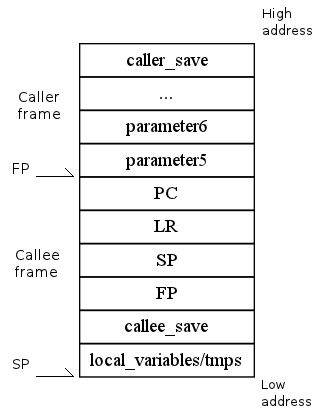
\includegraphics[scale=0.6]{stack_frame.png}
	\label{fig:stackframe}
\end{center}
\end{minipage}
\begin{minipage}{0.4\textwidth}
\begin{center}
	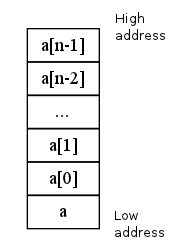
\includegraphics[scale=0.6]{local_array.png}
	\label{fig:localarray}
\end{center}
\end{minipage}
\captionof{figure}{栈帧与局部数组示意图}
\end{center}
FP以上(高地址方向)是调用者的部分栈帧(略去部分和被调用者栈帧相似),其中保存了call save寄存器以及传给被调用者的从第5个到最后一个参数(如果被调用者参数小于等于4,那么省去这一段)。

FP到SP的一段是被调用者的栈帧,其中保存了调用时的PC,返回地址,调用者的栈顶地址和栈帧基址以及callee save寄存器的值。同时,每一个局部变量和没有分配寄存器的临时变量在栈帧中均有位置。


\subsubsection{全局区的维护以及大立即数的处理}
我们将全局变量(或数组)、字符串常量保存在全局区中。由于全局区可能较大,使用基址和偏移量的寻址方式很可能出现偏移量过大不能使用带立即数的访存指令的问题。为此,我们将每个函数需要用到的全局变量的指针保存在该函数的代码段末尾,并分配给它们一个标号。当使用这些标号寻址时,汇编器会自动将寻址方式转换成PC相对寻址。

对于无法使用立即数寻址的三元式中的立即数,我们也将它保存在函数的代码段末尾,通过PC相对寻址将其读入。

例如下述代码:
\begin{lstlisting}
int a,b;
int f()
{
	a=25500;
	b=25500;
}

\end{lstlisting}
我们将生成如下的汇编代码:
\begin{verbatim}
	TODO: assemble code
\end{verbatim}
\section{寄存器分配}

\section{将三元式转换为目标代码}

\section{机器相关优化}
\subsection{尾递归优化}
\subsection{窥孔优化}
